\documentclass[a4paper]{article}
\usepackage{hyperref}
\usepackage[ngerman]{babel}
\usepackage{amsmath}
\usepackage{amsfonts}
\usepackage{amsthm}
\usepackage{tcolorbox}
\usepackage[a4paper,left=2cm,right=2cm,top=2.5cm,bottom=2.5cm]{geometry}
\usepackage[font={scriptsize,it}]{caption}
\usepackage{scrextend}
\usepackage{graphicx}
\usepackage{caption}
\usepackage{subcaption}
\usepackage[utf8]{inputenc}
\usepackage[T1]{fontenc}
\DeclareUnicodeCharacter{2212}{-}
\usepackage{verbatim}
\usepackage{tikz}

\tikzset{
  treenode/.style = {shape=rectangle, rounded corners,
                     draw, align=center,
                     top color=white, bottom color=blue!20},
  root/.style     = {treenode, font=\Large, bottom color=red!30},
  env/.style      = {treenode, font=\ttfamily\normalsize},
  dummy/.style    = {circle,draw}
}

\tikzstyle{level 1}=[level distance=3.5cm, sibling distance=3cm]
\tikzstyle{level 2}=[level distance=3.5cm, sibling distance=2cm]

% floating figure for column
\newenvironment{Figure}
	{\par\medskip\noindent\minipage{\linewidth}}
	{\endminipage\par\medskip}

\theoremstyle{definition}
\newtheorem{definition}{Definition}
 
\theoremstyle{example}
\newtheorem*{example}{Example}

\begin{document}

%\begin{titlepage}
%  \vspace*{\stretch{1.0}}
 % \begin{center}
%      \Large\textbf{MANIT3 - HS19}\\
%      \large\textit{Pascal Brunner - brunnpa7}
%   \end{center}
%  \vspace*{\stretch{2.0}}
%\end{titlepage}



\section{Einführung Stochastik}
Grundsätzlich befasst sich die Stochastik mit Aussagen, welche nicht sicher sind. Sprich nicht klar, ob wahr oder falsch. Dabei wird unteranderem die Aussagelogik und die Mengenlehre einen Teil davon sein.

%Deskriptiv ist nicht Prüfungsrelevant

\section{unsichere Ereignisse}

Die \textbf{Wahrscheinlichkeit} wird zwischen 0 $\leq$ P $\leq$ 1. Wobei 0 $\equiv$ unmöglich und 1 $\equiv$ sicher
Wahrscheinlichkeiten welche wir vergeben sind Ereignisse $A \subset \Omega$. 
P({K}), das heisst Einzelereignisse werden \textbf{elementar Ereignisse} genannt.

\theoremstyle{definition}
\begin{tcolorbox}
\begin{definition}
Es sei $\Omega$ die Menge aller möglichen Ergebnisse eines unsicheren Vorgangs. Ein Ergebnis ist eine Teilmenge von $\Omega$.
\begin{enumerate}
\item{Für jedes Ereignis A ist die Wahrscheinlichkeit von A, genannt P(A), eine reelle Zahl zwischen 0 und 1: 0 $\equiv$ P(A) $\equiv$ 1}
\item{$P(\Omega)=1$}
\item{Falls A und B disjunkt, dann $P(A \cup B) = P(A) + P(B)$}
\end{enumerate}
\end{definition}
\end{tcolorbox}

\theoremstyle{definition}
\begin{tcolorbox}
\begin{definition}
\textbf{Ergebnisse vs. Ereignisse}
\begin{itemize}
\item \textbf{Ergebnisse} sind alle $\Omega = {k,z}$
\item \textbf{Ereignisse} sind alle Teilmengen von $\Omega$ und für alle dieser Teilmengen wird eine Wahrscheinlichkeit zugeordnet
\item \textbf{elementar Ereignis} sind alle Kombination $P({...}) = \frac{1}{|\Omega|}$
\end{itemize}
\end{definition}
\end{tcolorbox}


\subsubsection{Beispiel unsichere Ereignisse anhand eines Münzwurfs}
\textit{Der unsichere Ausgang eines einzelnen Münzwurfs hat die Ergebnismenge $\Omega ={Zahl,Kopf}$ $\rightarrow$ $|Omega|=2$} $\Rightarrow$ wird Mächtigkeit von $\Omega$ genannt\\
Dabei hat man folgende Teilmengen: \{\},\{K\},\{Z\},\{K,Z\}. Jeder Teilmenge ordnet man nun eine Wahrscheinlichkeit P zu.\\ $\rightarrow$ $P({K})=0.5, P({Z})=0.5, P({})= 0\textrm{ und }P({K,Z})=1$. Denn $P({K,Z})$ ist eine \textbf{disjunkte Teilmenge}. Gemäss Definition bedeutet dies Kopf oder Zahl, was in diesem Beispiel immer zutrifft.

\section{Wahrscheinlichkeit und Kombinatorik}
%tbd

\subsection{Beispiele zur Wahrscheinlichkeit und Kombinatorik}
\subsubsection{Kino-Plätze belegen mit unterschiedlichen Gruppen}
\textit{Wir haben zwei Gruppen\\ Gruppe 1 $=$ 5 Personen, Gruppe 2 $=$ 4 Personen, Insgesamt = 9 Personen}\\
\textit{Frage 1: Wie viele Möglichkeiten gibt es, wie die 9 Personen sitzen können?}\\
$\Rightarrow = 9! \rightarrow 9$ Fakultät $\rightarrow 9*8*7*...*1$\\
\textit{Frage 2: Wie viele Möglichkeiten gibt es, wenn die Gruppen nebeneinander sitzen müssen?}\\
$\Rightarrow$ Möglichkeit 1: $\underbrace{P1 P2 P3 P4 P5}_{\substack{Gruppe 1}} * \underbrace{P6 P7 P8 P9}_{\substack{Gruppe 2}} \rightarrow = 5! * 4!$\\
$\Rightarrow$ Möglichkeit 2: $\underbrace{P1 P2 P3 P4}_{\substack{Gruppe 2}} * \underbrace{P5 P6 P7 P8 P9}_{\substack{Gruppe 1}} \rightarrow = 4! * 5!$\\
\textbf{merke: } Möglichkeit 1 ist zur Möglichkeit 2 \underline{disjunkt}\\
Also ist die Lösung: $|\Omega| = |\Omega_1| + |\Omega_2| = 2*5!*4!$

\textit{Frage 3: Wie sieht die Berechnung aus, wenn nun noch eine weitere Gruppe mit 6 Personen dazu kommt?}\\
Ich habe nun $3!$ Möglichkeiten die Gruppen grundsätzlich zu platzieren. Anschliessend gibt es innerhalb der Gruppen wieder $n!$ (Anzahl Personen in Gruppe) Möglichkeiten die Platzierung vorzunehmen.\\
Also ist die Lösung: $\Rightarrow \underbrace{3!}_{\substack{\textrm{Anordnung der Gruppen}}} * \underbrace{5!}_{\substack{\textrm{Anordung Gruppe 1}}} * \underbrace{4!}_{\substack{\textrm{Anordnung Gruppe 2}}} * \underbrace{6!}_{\substack{\textrm{Anordnung Gruppe 3}}}$

\subsubsection{Zählprinzip gezeigt anhand von Lottozahlen}
\textit{Wir kreuzen 6 Lottozahlen von 49 möglichen Zahlen an}\\
$\rightarrow$ wir entscheiden uns für die Zahlen 2, 5, 10, 43, 44, 47. Dies sieht als Tupel wie folgt aus $(2, 5, 10, 43, 44, 47)$\\
\textit{Frage 1: Berechnung der Wahrscheinlichkeit mit Reihenfolge}\\
$\underbrace{49}_{\substack{\textrm{1. Wahl}}} * \underbrace{48}_{\substack{\textrm{2. Wahl}}} * \underbrace{47}_{\substack{\textrm{3. Wahl}}} * \underbrace{46}_{\substack{\textrm{4. Wahl}}} * \underbrace{45}_{\substack{\textrm{5. Wahl}}} * \underbrace{44}_{\substack{\textrm{6. Wahl}}} \Rightarrow 49 * 48 * 47 * 46 * 45 * 44$\\\\
\textit{Frage 2: Bei der Wahl der Lottozahlen ist die Reihenfolge, wie die Zahlen angekreuzt wurden irrelevant. Aus diesem Grund müssen wir einen Korrekturfaktor berechnen.}\\
Hierzu gibt es folgendes Vorgehen:
\begin{enumerate}
\item Tue so als ob es sich um eine Berechnung mit Reihenfolge handelt (Beispiel Frage 1)
\item Berechne wie viele Möglichkeiten, dass es gibt, wie die Zahlen angekreuzt werden.
\item Teile die Resultat $\frac{1.)}{2.)} $
\end{enumerate}
Der erste Schritt haben wir bereits in der Frage 1 beantwortet. Für die Frage 2, stellen wir fest, dass es  $6!$ Möglichkeiten gab. Nun teilen wir dies durch das Resultat von Frage 1 und erhalten:
$\frac{49 * 48 * 47 * 46 * 45 * 44}{6!}$

\subsubsection{Wörter}
\textit{Gegeben ist ein Wort $\rightarrow$ STATISTIK}
Nun berechnen wir wie im vorherigen Beispiel gezeigt zuerst den Wert aus, wenn es sich um eine Reihenfolge handelt. Wir haben 9 Buchstaben im Wort STATISTIK, also entspricht dies $9!$.\\
Nun stellen wir fest, dass es mehrere Buchstaben gibt, welche identisch sind im Wort.\\
$S_1T_1AT_2I_1S_2T_3I_2K$ $\Rightarrow$ Wir erhalten damit einen Korrekturfaktor von $\underbrace{3!}_{\substack{T's}}*\underbrace{2!}_{\substack{S's}}*\underbrace{2!}_{\substack{I's}}$\\
Entsprechend teilen wir die beiden Teilergebnisse um $|\Omega|$ zu erhalten.\\
$|\Omega| = \frac{9!}{3!*2!*2!}$ Der Kehrwert von $|\Omega|$ ist entsprechend die Wahrscheinlichkeit $=\frac{1}{|\Omega|}$

\subsubsection{Kontext für weitere Berechnungen}
Aus den vorherigen Beispielen haben wir die Wahrscheinlichkeit erhalten, doch wie kann ich damit rechnen?\\
Wir illustrieren dies anhand eines zweifachen Münzwurfes (wobei $K=Kopf, Z=Zahl, M_n =$ n-ter Münzwurf darstellt:\\
$\Omega = \{(K,K), (K,Z), (Z,K), (Z,Z)\}$\\
\textit{Wir möchten nun einmal Kopf erhalten:}\\
Genauer betrachtet stellen wir fest, dass es keine Rolle spielt ob wir nun im ersten oder zweiten Wurf eine Kopf werfen. $\rightarrow \{(K,Z)\} \underbrace{\cup}_{\substack{oder}} \{(Z,K)\} \Rightarrow M_1 \cup M_2 = \{x | x \in M_1 \vee x \in M_2\}$
\begin{Figure}
\centering
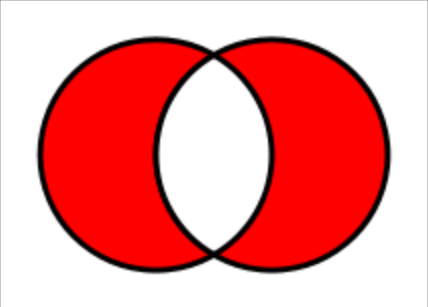
\includegraphics[width=100px]{img/keineSchnittmenge.png}
	\captionof{figure}{Abbildung ODER, wenn keine Schnittmengen bestehen}
	\label{fig:keine Schnittmengen}
\end{Figure}

Hingegen ist eine Schnittmenge wie folgt definiert:
$A \cap B = \{x | x \in A \wedge x \in B\}$\\
Wann immer wir von $P(A,B)$ sprechen ist wichtig zu wissen, dass dies $P(A \wedge B)$ bedeutet.
\begin{Figure}
\centering
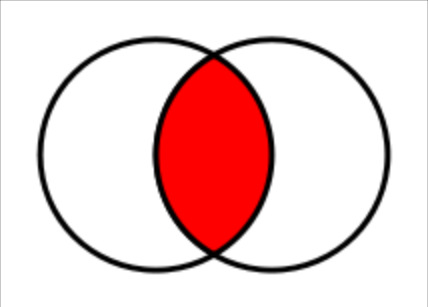
\includegraphics[width=100px]{img/Schnittmenge.png}
	\captionof{figure}{Abbildung UND, wenn Schnittmengen bestehen}
	\label{fig:Schnittmengen}
\end{Figure}

\subsection{Beispiele für zwei Ereignisse}
Wir schauen uns nun einige Beispiele an für die Berechnung mit zwei Ereignisse und leiten daraus unsere Erkenntnisse ab.
\subsubsection{doppelter Münzwurf}
Kehren wir zu unserem zweifachen Münzwurf zurück. Diese Wahrscheinlichkeiten lassen sich nun auch in Tabellen Form darstellen.\\

\begin{table}[h!]
	\begin{center}
		\caption{zweifacher Münzwurf in Tabellenform}
		\label{tab: table1}
		\begin{tabular}{c|c|c}
			\textbf{P} & \textbf{K} & \textbf{Z}\\
			\hline
			\textbf{K} & $P(W_1=K, W_2=K)$ & $P(W_1=K, W_2=Z)$\\
			\textbf{Z} & $P(W_1=Z, W_2=K)$ & $P(W_1=Z, W_2=Z)$	
		\end{tabular}
	\end{center}
\end{table}

Betrachten wir den zweifachen Münzwurf, haben wir die Wahrscheinlichkeiten der einzelnen Kombinationen gegeben, diese fügen wir nun der Tabelle ein.
\begin{table}[h!]
	\begin{center}
		\caption{zweifacher Münzwurf in Tabellenform inkl. Marginalisierung}
		\label{tab: table1}
		\begin{tabular}{c|c|c|c}
			\textbf{P} & \textbf{K} & \textbf{Z} & \textbf{$\sum$}\\
			\hline
			\textbf{K} & 0.49 & 0.21 & $= 0.7$\\
			\textbf{Z} & 0.21 & 0.09 & $= 0.2$\\
			\textbf{$\sum$} & $= 0.7$ & $= 0.3$\\
		\end{tabular}
	\end{center}
\end{table}
Das $\sum$ steht für das sogenannte \textbf{Marginalisieren}. Wir berechnen jeweils die Spaltensumme, sowie die Zeilensumme und schreiben dies am Ende der Tabelle hin. \\
\textbf{Fundamentale Erkenntnisse:}\\
\textbf{Unabhängigkeit} anhand des Beispiels mit dem doppelten Münzwurf.\\

$P(W_1 = K, W_2 = K) = P(W_1 = K) * P(W_2 = K)  \rightarrow$ Die Randwahrscheinlichkeiten $0.7*0.7 = 0.49$ multipliziert, gibt das Ergebnis im Inneren. Aus dem erhalten wir die Feststellung, dass $W_1 = K$ und $W_2 = K$ \textbf{unabhängig} voneinander sind $\rightarrow$ Ich sage das Ergebnis für das Erste, dies beinflusst die Wahrscheinlichkeit für das zweite \underline{nicht}.

\subsubsection{Konsum von Alkohol und Zigaretten bei Teenagern}
\textit{Frage: Bestimmen Sie durch Marginalisierung jeweils die Wahrscheinlichkeit der einzelnen Ereignisse aus den Wahrscheinlichkeiten der gemeinsamen Ereignisse}\\
Gegeben sind folgende Informationen:\\
\begin{table}[h!]
	\begin{center}
		\caption{Abhängigkeit zwischen Alkohol- und Zigaretten Konsum bei Teenagern}
		\label{tab: table1}
		\begin{tabular}{c|c|c}
			\textbf{P} & \textbf{Trinkt Alkohol (A)} & \textbf{Trinkt kein Alkohol ($\mathbf{\bar{A}}$)}\\
			\hline
			\textbf{Raucht Zigaretten (Z)} & 0.56 & 0.01\\
			\textbf{Raucht keine Zigaretten ($\mathbf{\bar{Z}}$)} & 0.25 & 0.18
		\end{tabular}
	\end{center}
\end{table}

Als erstes berechnen wir nun wieder die Spalten- und Zeilensummen (auch Randsummen genannt):\\
\begin{table}[h!]
	\begin{center}
		\caption{Abhängigkeit zwischen Alkohol- und Zigaretten Konsum bei Teenagern}
		\label{tab: table1}
		\begin{tabular}{c|c|c|c}
			\textbf{P} & \textbf{Trinkt Alkohol (A)} & \textbf{Trinkt kein Alkohol ($\mathbf{\bar{A}}$)} & \textbf{$\sum$}\\
			\hline
			\textbf{Raucht Zigaretten (R)} & 0.56 & 0.01 & $P(R) = 0.57$\\
			\textbf{Raucht keine Zigaretten ($\mathbf{\bar{R}}$)} & 0.25 & 0.18 & $P(\bar{R} = 0.43$\\
			\textbf{$\sum$} & $P(A) = 0.81$ & $P(\bar{A}) = 0.19$\\
		\end{tabular}
	\end{center}
\end{table}
Daraus können wir unsere ersten Erkenntnisse schliessen:\\
\begin{itemize}
	\item Die Randsummen betrachten nur einen Faktor
	\item Die Zahl \textit{in der Mitte} betrachtet \textit{alle Faktoren}
	\item $\rightarrow$ aus den Randsummen lässt sich nicht auf die Mitte schliessen bzw. man kann es nicht rekonstruieren
\end{itemize}
\textbf{Fundamentale Erkenntnisse:}\\
\textbf{Abhängigkeit} anhand des Beispiels Alkohol- und Zigarettenkonsum.
\begin{itemize}
	\item {
	\textit{Sind R und A unabhängig?}
	\begin{equation}
	\begin{split}
		P(A) = 0.81 ; P(R) = 0.57 \\
		0.81 * 0.57 \stackrel{?}{=} 0.56
	\end{split}
	\end{equation}
	Daraus erhalten wir die Info, dass es sich um eine Abhängigkeit handelt, denn $0.81 * 0.57 \neq 0.56$ \\
	$\rightarrow$ es ist abhängig, dementsprechend beeinflusst das eine Ereignis, das andere
	}
\end{itemize}

\subsection{Bedingte Wahrscheinlichkeit}
Nun schauen wir uns die bedingte Wahrscheinlichkeit anhand des Alkohol, Zigaretten Beispiel an:\\
\textit{Gegeben ist A} (geschrieben als $|A$) $\Rightarrow$ Dies bedeutet, dass A sicher ist.\\
Die Tabelle, wenn A gegeben ist, sieht wie folgt aus:\\
\begin{table}[h!]
	\begin{center}
		\caption{bedingte Wahrscheinlichkeit zwischen Alkohol- und Zigaretten Konsum bei Teenagern wenn A gegeben ist}
		\label{tab: table1}
		\begin{tabular}{c|c|c}
			\textbf{P} & \textbf{A} & \textbf{$\sum$}\\
			\hline
			\textbf{R} & 0.56 & $P(\underbrace{R}_{\substack{unsicher}} | \underbrace{A}_{\substack{sicher}})$\\[15pt]
			\textbf{$\mathbf{\bar{R}}$} & 0.25 & $P(\underbrace{\bar{R}}_{\substack{unsicher}} | \underbrace{A}_{\substack{sicher}})$
		\end{tabular}
	\end{center}
\end{table}
Wir haben gelernt, dass die \textit{Mitte} in der Summe immer 1 geben muss. Dies ist jetzt nun jedoch nicht mehr der Fall. Aus diesem Grund müssen wir die Werte in der Tabelle der neuen Situation anpassen. \\
\begin{tcolorbox}
\begin{definition}[\textbf{bedingte Wahrscheinlichkeit}]
Die bedingte Wahrscheinlichkeit ist in diesem Fall gegeben durch:
\begin{equation}
P(R|A) = \frac{P(R,A)}{P(A)}
\end{equation}
Dadurch erhalten wir wieder eine \textit{echte} Wahrscheinlichkeit
\end{definition}
\end{tcolorbox}
\newpage
Entsprechend der neuen Definition führen wir nun die Korrektur aus und erhalten so in der Summe wieder 1:\\
\begin{table}[h!]
	\begin{center}
		\caption{Korrigierte bedingte Wahrscheinlichkeit wenn A gegeben ist}
		\label{tab: table1}
		\begin{tabular}{c|c|c}
			\textbf{P} & \textbf{A} & \textbf{$\sum$}\\
			\hline
			\rule{0pt}{1.2\normalbaselineskip} \textbf{R} & $\frac{0.56}{0.81} = 0.70$ & $P(\underbrace{R}_{\substack{unsicher}} | \underbrace{A}_{\substack{sicher}})$\\[15pt]
			\textbf{$\mathbf{\bar{R}}$} & $\frac{0.25}{0.81} = 0.30$ & $P(\underbrace{\bar{R}}_{\substack{unsicher}} | \underbrace{A}_{\substack{sicher}})$
		\end{tabular}
	\end{center}
\end{table}

Analog können wir diesen Prozess durchführen, wenn \textit{R} gegeben ist. An dieser Stelle berechnen wir es sogleich mit dem Korrekturfaktor:\\

\begin{table}[h!]
	\begin{center}
		\caption{Korrigierte bedingte Wahrscheinlichkeit wenn R gegeben ist}
		\label{tab: table1}
		\begin{tabular}{c|c|c}
			\textbf{P} & \textbf{A} & \textbf{$\mathbf{\bar{A}}$}\\
			\hline
			\rule{0pt}{1.2\normalbaselineskip} \textbf{R} & $\frac{0.56}{0.57} = 0.99$ & $\frac{0.01}{0.57} = 0.01$\\[15pt]
			\textbf{$\sum$} & $P(\underbrace{A}_{\substack{unsicher}} | \underbrace{R}_{\substack{sicher}})$ & $P(\underbrace{\bar{A}}_{\substack{unsicher}} | \underbrace{R}_{\substack{sicher}})$
		\end{tabular}
	\end{center}
\end{table}

%\begin{tcolorbox}
%\begin{definition}[\textbf{mathematischer Beweis: Wenn eine Unabhängigkeit besteht, dann sind alle unabhängig (in einer 2x2 Tabelle)}]
%Der Mathematische Beweis ist \underline{nicht Prüfungsrelevant}
%\textit{Gegeben: } A,B sind unabhängig $\Rightarrow P(A,B) = P(A) * P(B)$\\
%\textit{Gesucht: } Wenn eines unabhängig ist, dann sind alle unabhängig.
%\begin{equation}
%	\begin{split}
%		\Rightarrow P(A, \bar{B}) &\stackrel{?}{=} P(A) * P(B) \\
%		 1.) \quad P(A,B) + P(A,\bar{B}) &= P(A) \\
%		 2.) \quad P(A) * P(B) + P(A, \bar{B}) &= P(A) \quad A, B \Rightarrow unabh.\\
%		 3.) \quad \underline{P(A, \bar{B})} &= P(A) - P(A)*P(B) = P(A) * (1-P(B)) = \underline{P(A) * P(\bar{B})}
%	\end{split}
%\end{equation}
%Dadurch erhalten wir wieder eine \textit{echte} Wahrscheinlichkeit
%\end{definition}
%\end{tcolorbox}

\subsubsection{Baum-Darstellung}
Nicht immer ist die Tabellenform die geeigneste Form für die Darstellung. Ein Baum ist ebenfalls ein häufig eingesetztes Mittel um die Sequenz entsprechend darzustellen. Nachfolgend ist der Baum ersichtlich, wenn A gegeben ist:\\
\begin{center}
	\begin{tikzpicture}
	  [
	    grow                    = right,
	    sibling distance        = 6em,
	    level distance          = 6em,
	    edge from parent/.style = {draw, -latex},
	    every node/.style       = {font=\footnotesize},
	    sloped
	  ]
	  \node [root] {Formula}
		child{
			node [dummy] {}
			child{
				node[env]{$\bar{R} | \bar{A} = xx.xx$}
				edge from parent node [above]{$P(\bar{R} | \bar{A})$}
			}		
			child{
				node[env]{$R | \bar{A} = xx.xx$}
				edge from parent node [above]{$P(R | \bar{A})$}
			}
			edge from parent 
	            node[above] {$\bar{A}$}
		}  	
	  	child{
	  		node [dummy] {}
			child{
				node[env]{$\bar{R} | A = xx.xx$}
				edge from parent node [above]{$P(\bar{R} | A)$}
			}		
			child{
				node[env]{$R | A = xx.xx$}
				edge from parent node [above]{$P(R | A)$}
			}
			edge from parent 
	            node[above] {$A$}
		}
		;
	\end{tikzpicture}
\end{center}

\subsection{Zusammenfassung}
Wir fassen unsere Kenntnisse anhand eines neuen Beispiels zusammen. Wir betrachten den Zusammenhang zwischen Menschen die Hunde mögen und Menschen die Katzen mögen.
\begin{table}[h!]
	\begin{center}
		\caption{Abhängigkeit zwischen Hunde- und Katzenliebhaber}
		\label{tab: table1}
		\begin{tabular}{c|c|c}
			\textbf{P} & \textbf{Mag Hunde (H)} & \textbf{Mag keine Hunde($\mathbf{\bar{H}}$)}\\
			\hline
			\textbf{Mag Katzen (K)} & 0.15 & 0.3\\
			\textbf{Mag keine Katzen($\mathbf{\bar{K}}$)} & 0.25 & 0.3
		\end{tabular}
	\end{center}
\end{table}
\begin{itemize}
	\item {Randwahrscheinlichkeiten
		\begin{enumerate}
			\item $P(K)$
			\item $P(H)$
		\end{enumerate}			
	}
	\item {bedingte Wahrscheinlichkeiten
		\begin{enumerate}
			\item $P(K|H)$
			\item $P(K|\bar{H})$
			\item $P(H|K)$
			\item $P(H|\bar{K})$
		\end{enumerate}
	}
	\item {gemeinsame Wahrscheinlichkeit
		\begin{enumerate}
			\item $P(H,K) = P(K,H)$
		\end{enumerate}
	}
	\item{Unabhängigkeit
		\begin{enumerate}
			\item $P(K) = P(K|H)$
			\item $P(\bar{K}) = P(\bar{K}|H)$
			\item $P(H) = P(H|K)$
			\item $P(\bar{H} = P(\bar{H}|K)$
		\end{enumerate}
		$\Rightarrow$ Bei Unabhängigkeit gilt: $P(H)*P(K) = P(K,H)$
	}
\end{itemize}

\section{Satz von Bayes}
Wir veranschaulichen den Satz von Bayes anhand eines weiteren Beispiels:\\
\textit{Ein Tourist wird beim Arzt auf eine Krankheit getestet, die in etwa bei jedem tausendsten in seinem Land vorkommt. Der Tests diagnostiziert 99\% der Kranken korrekt. Allerdings werden auch 2\% der gesunden Menschen fälschlicherweise als krank diagnostiziert. Laut Test ist der Tourist krank; mit welcher Wahrscheinlichkeit muss er sich wirklich Sorgen machen?}\\
Aus der Aufgabenstellung erhalten wir folgende Informationen:\\
\begin{itemize}
	\item $P(K) = \frac{1}{1000}$
	\item $P(T|K) = 0.99$
	\item $P(T|\bar{K}) = 0.2$
	\item $P(K|T) =$ \textbf{gesucht}
\end{itemize}
Hierbei stellen wir schnell fest, dass die Tabelle kein sehr hilfreiches Instrument ist. Die Tabelle ist vor allem hilfreich, wenn man die bedingte Wahrscheinlichkeit hat. Daher zeichnen wir das ganze einmal als Baum auf:\\

\begin{Figure}
\centering
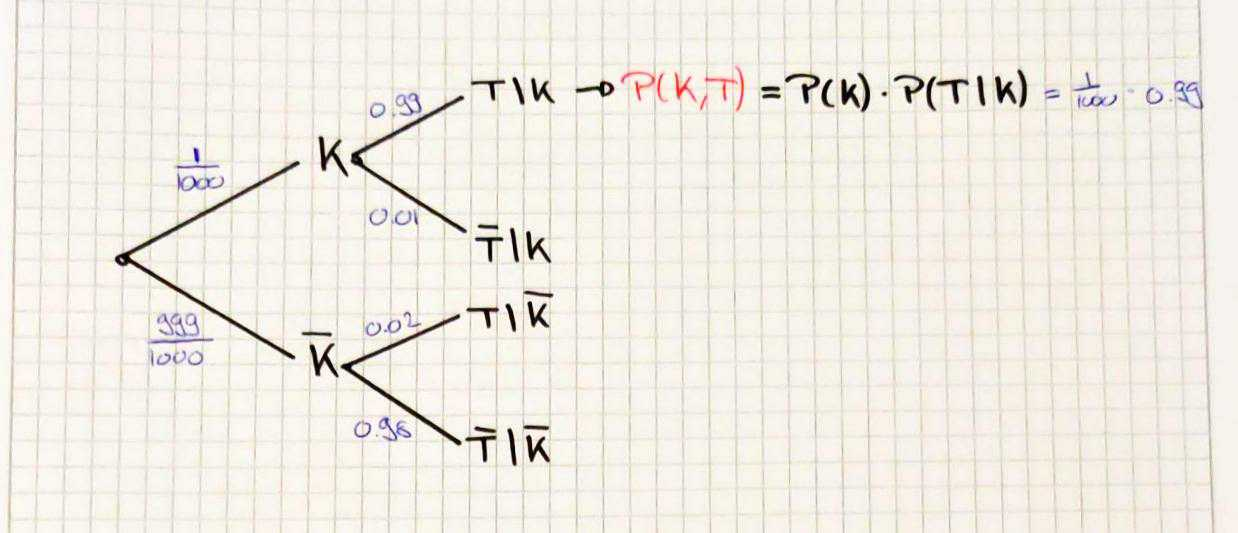
\includegraphics[width=200px]{img/BaumKgegeben.jpg}
	\captionof{figure}{Baum inkl. Wsk wenn K gegeben}
	\label{fig:Baum inkl. Wsk wenn K gegeben}
\end{Figure}

Anhand des Baumes stellen wir fest, dass wir im obersten Ast $P(T|K)$ erhalten. Dies wiederum ist definiert als die gemeinsame Wahrscheinlichkeit $P(K,T) = P(K)*P(T|K)$\\
Daraus können wir folgende Umformung vornehmen:\\
\begin{equation}
P(K|T) = \frac{P(K,T)}{P(T)} = \frac{\frac{1}{1000}*0.99}{\underbrace{\frac{1}{1000}*0.99}_{\substack{P(T,K)}}+\underbrace{\frac{999}{1000}*0.02}_{\substack{P(T,\bar{K})}}} = 0.047
\end{equation}

Dies ist auch mit dem Baum, wenn T gegeben ist, ersichtlich:\\

\begin{Figure}
\centering
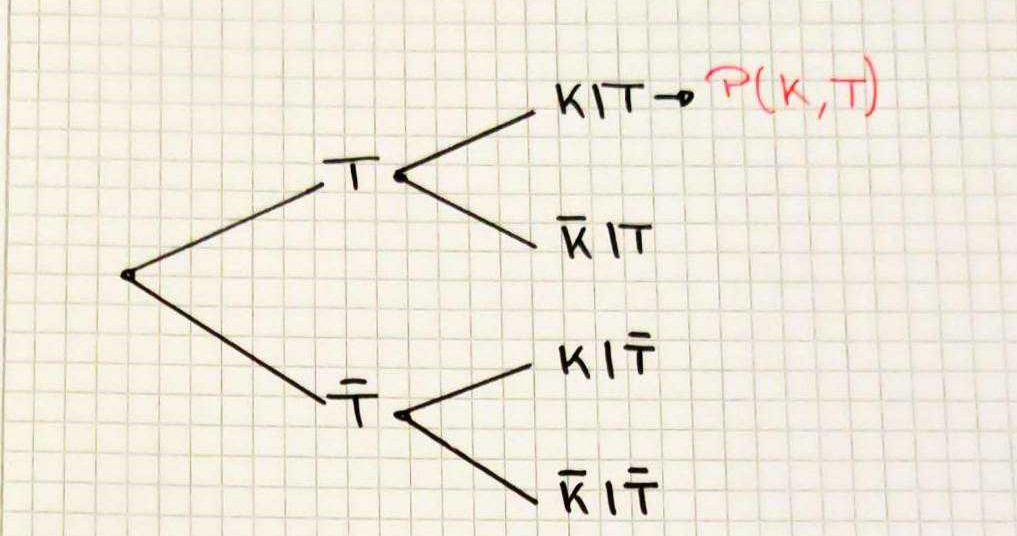
\includegraphics[width=200px]{img/BaumTgegeben.jpg}
	\captionof{figure}{Baum inkl. Wsk wenn T gegeben}
	\label{fig:Baum inkl. Wsk wenn T gegeben}
\end{Figure}

\textbf{erste Erkenntnisse:}
\begin{enumerate}
	\item {Wenn der Arzt sagt, dass man krank ist, stimmt dies nur zu 4.7\%}
	\item {Zwei Faktoren spielen dabei mit:
		\begin{itemize}
			\item sehr seltene Krankheit
			\item 0.02 Fehler
		\end{itemize}
	}
	\item {Möglichkeiten zur Verbesserung:
		\begin{itemize}
			\item Test verbessern
			\item zweiter Test
		\end{itemize}
	}
\end{enumerate}


\begin{tcolorbox}
	\begin{definition}[\textbf{Satz von Bayes}]
	\textit{Gegeben: } $P(T|K)$ bzw. $P(K,T)$\\
	\textit{Gesucht: } $P(K|T)$
		\begin{equation}
			\begin{split}
				\Rightarrow P(K,T) &= P(T) * P(K|T)\\
				P(T) * \underbrace{P(K|T)}_{\substack{gesucht}} &= \underbrace{P(K,T)}_{\substack{\textrm{equivalent zu }\frac{P(K)*P(T|K)}{P(T)}}} = P(K)*P(T|K)\\
				\underbrace{P(K|T)}_{\substack{\textrm{equivalent zu }P(T|K)}} &= \frac{P(K)*P(T|K)}{P(T)} = \frac{P(K,T)}{P(T)}\\
			\end{split}
	\end{equation}
	Wobei 
	Dieser Satz ist vor allem bei der Baumbetrachtung sehr verständlich.\\
\begin{Figure}
	\centering
	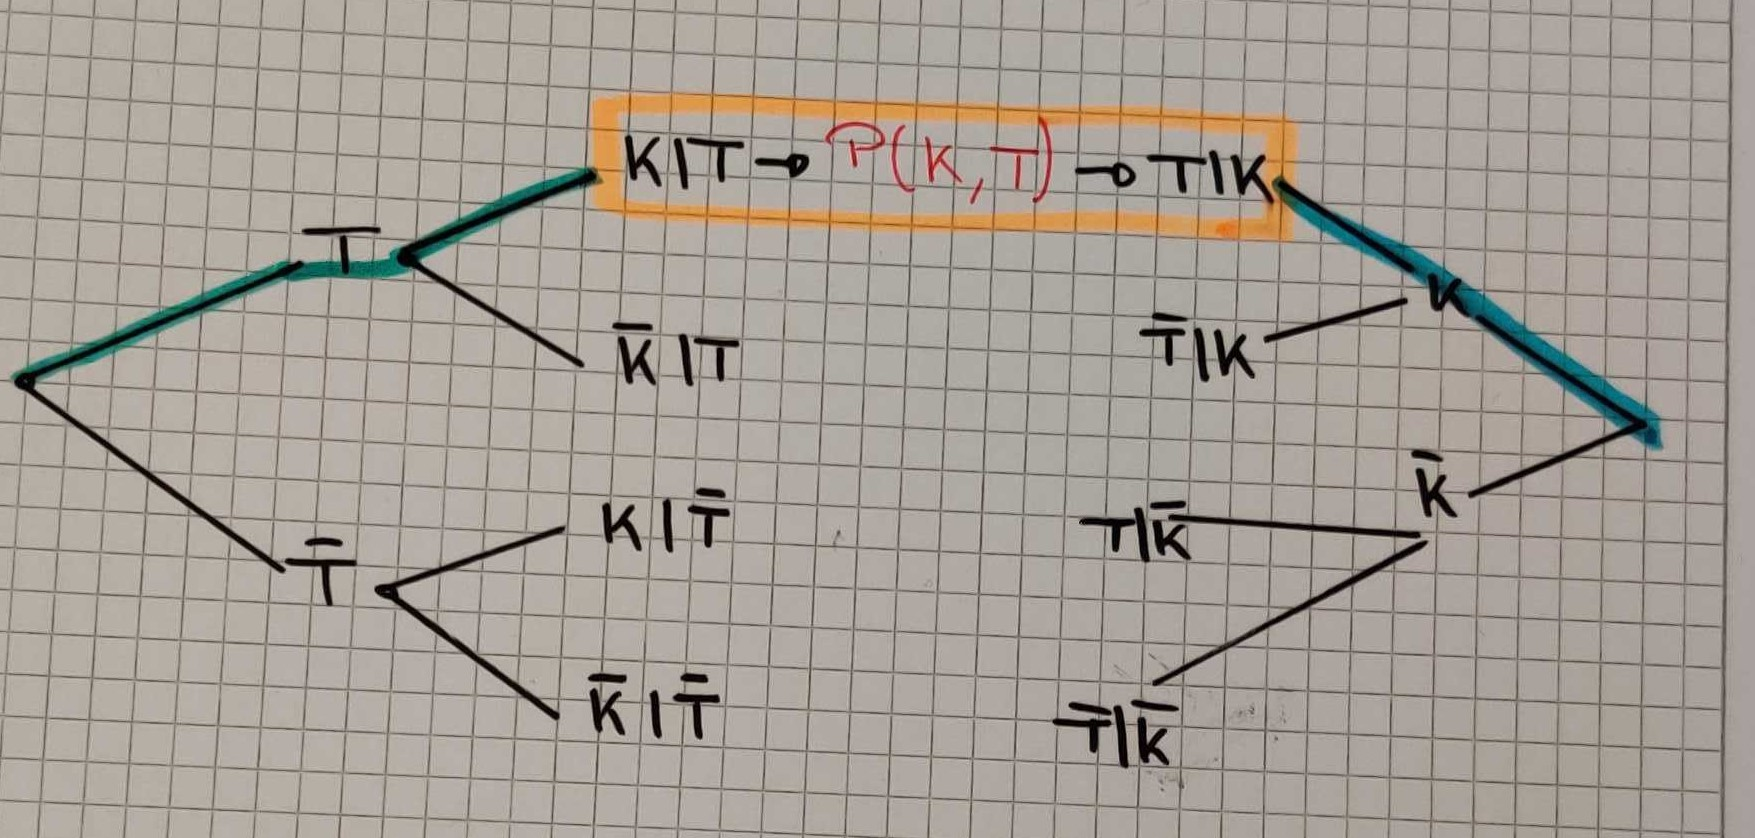
\includegraphics[width=200px]{img/BaumGegenueberstellung.jpg}
	\captionof{figure}{Baum T gegeben wird K gegeben gegenübergestellt}
	\label{fig:Baum T gegeben wird K gegeben gegenübergestellt}
\end{Figure}
	\end{definition}
\end{tcolorbox}

\subsection{Beispiele zum Satz von Bayes}

\subsubsection{Wahrscheinlichkeit, dass jemand tatsächlich ist, wenn der Test es sagt.}
In diesem Beispiel führen wir den Satz von Bayes ohne die Baumstruktur durch.\\
Folgendes ist gegeben:\\
\begin{equation}
\begin{split}
	P(K) &= 0.001 \\
	P(T | K) &= 0.99 \\
	P(T | \bar{K}) &= 0.02 \\
	P(K | T) = ?
\end{split}
\end{equation}
Wir wenden nun den Satz von Bayes an, damit wir von den gegebenen Informationen zum gesuchten $P( K | T)$ kommen:
\begin{equation}
	P(K|T) = \frac{P(T|K) * P(K)}{P(T)} = \frac{P(T|K) * P(K)}{\underbrace{P(T|K) * P(K)}_{\substack{P(T,K)}} + \underbrace{P(T|\bar{K}) * P(\bar{K})}_{\substack{P(T,\bar{K})}}}
\end{equation}
\textbf{merke: } Im dritten Gleichungsschritt haben wir immer der Zähler auch im Nenner

\subsubsection{Kugelziehen}
Wir haben zwei Beutel gegeben. Im ersten Beutel, befinden sich zwei schwarze Kugeln, im zweiten Beutel befindet sich eine schwarze und eine weisse Kugel.\\
\textit{1.) Mit welcher Wahrscheinlichkeit zieht man eine schwarze Kugel? $\rightarrow P(S)$}

\begin{Figure}
	\centering
	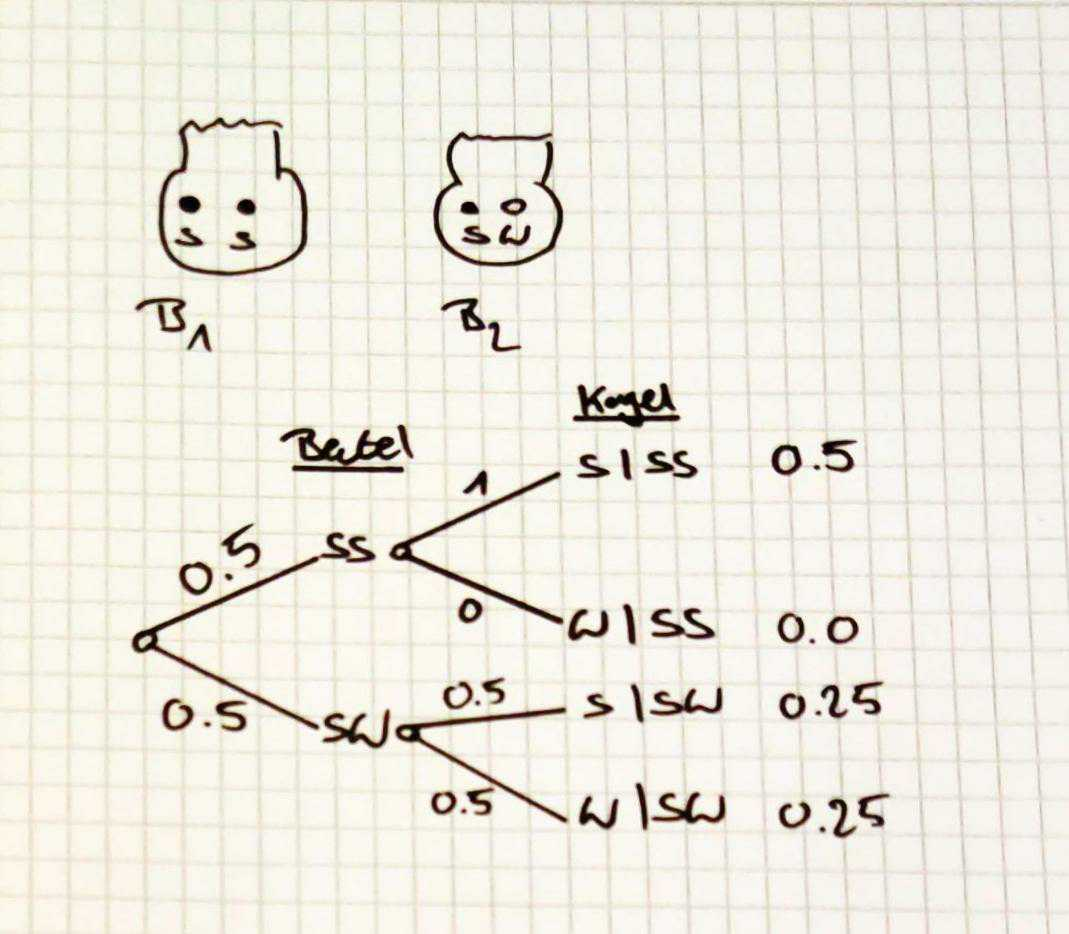
\includegraphics[width=100px]{img/SS_SW_Kugelziehen.jpg}
	\captionof{figure}{Wsk schwarze Kugel gezogen}
	\label{fig:Wsk schwarze Kugel gezogen}
\end{Figure}

\begin{equation}
 P(Kugel = S) = P(Beutel = SS, Kugel = S) + P(Beutel = SW, Kugel=S) = 0.5*1+0.5*0.5 = 0.75
\end{equation}

\textit{2.) Nun schaue ich die Kugel an und muss bestimmen aus welchem Beutel ich die Kugel gezogen habe?}\\
Dies machen wir wiederum mit dem Satz von Bayes

\begin{equation}
P(SS|S) = \frac{P(S|SS) * P(SS)}{P(S)} = \frac{0.5*1}{0.5*1 + 0.5*0.5} = \frac{0.5}{0.75} = \frac{2}{3}
\end{equation}

\textit{3.) Ich ziehe eine Kugel, lege Sie zurück und ziehe wieder aus dem gleichen Beutel eine Kugel. Mit welcher Wahrscheinlichkeit, habe ich welchen Beutel gezogen?}\\
Die Baumdarstellung lässt sich auf zwei Variante durchführen:\\
\textbf{Variante 1}\\
\begin{Figure}
	\centering
	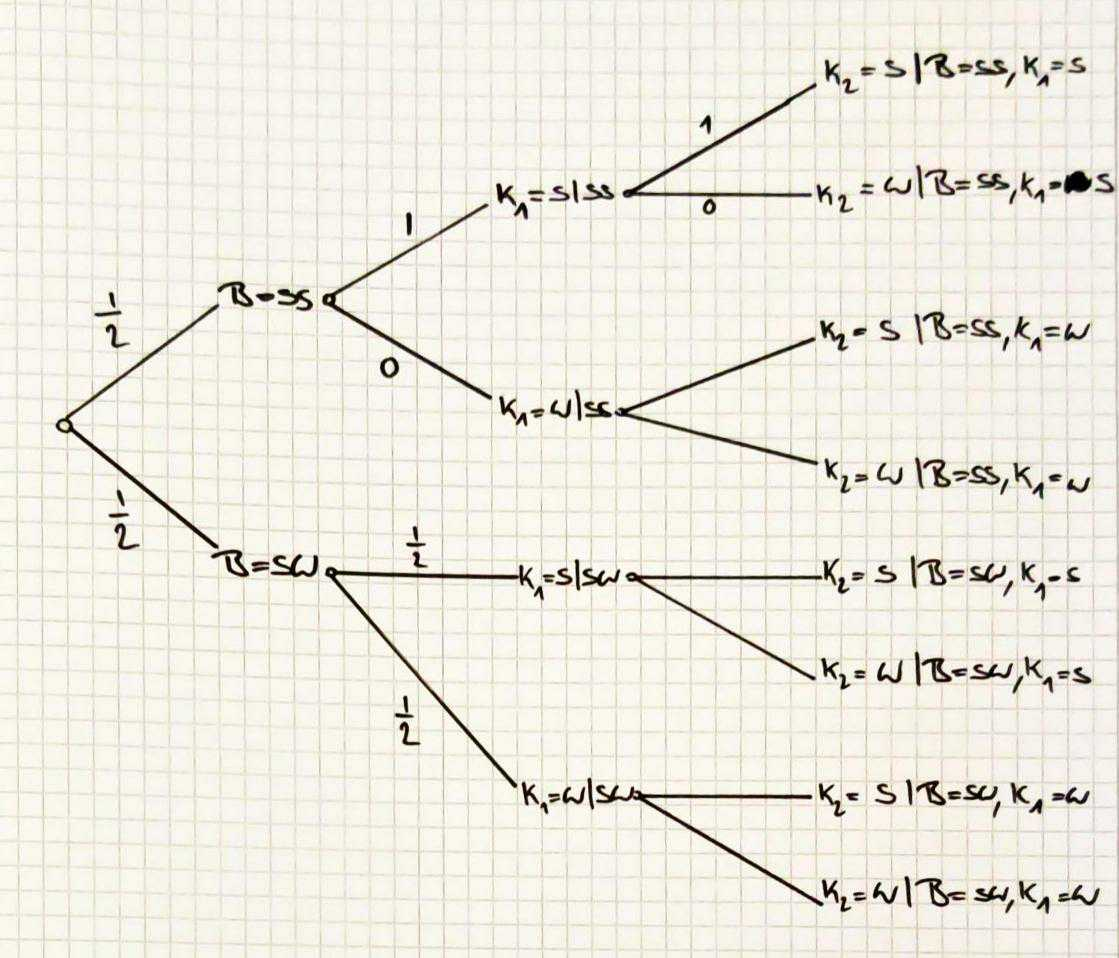
\includegraphics[width=100px]{img/MehrfachBaumVar1.jpg}
	\captionof{figure}{Variante 1 der Baum-Darstellung}
	\label{fig:Variante 1 der Baum-Darstellung}
\end{Figure}
\begin{equation}
P(B=SS | K_1 = S, K_2 = S) = \frac{P(B=SS, K_1=S, K_2=S)}{P(K_1=S,K_2=S)} = \frac{0.5*1*1}{0.5*1*1+0.5*0.5*0.5} = \frac{4}{5}
\end{equation}

\textbf{Variante 2 - Tupel-Darstellung}\\
\begin{Figure}
	\centering
	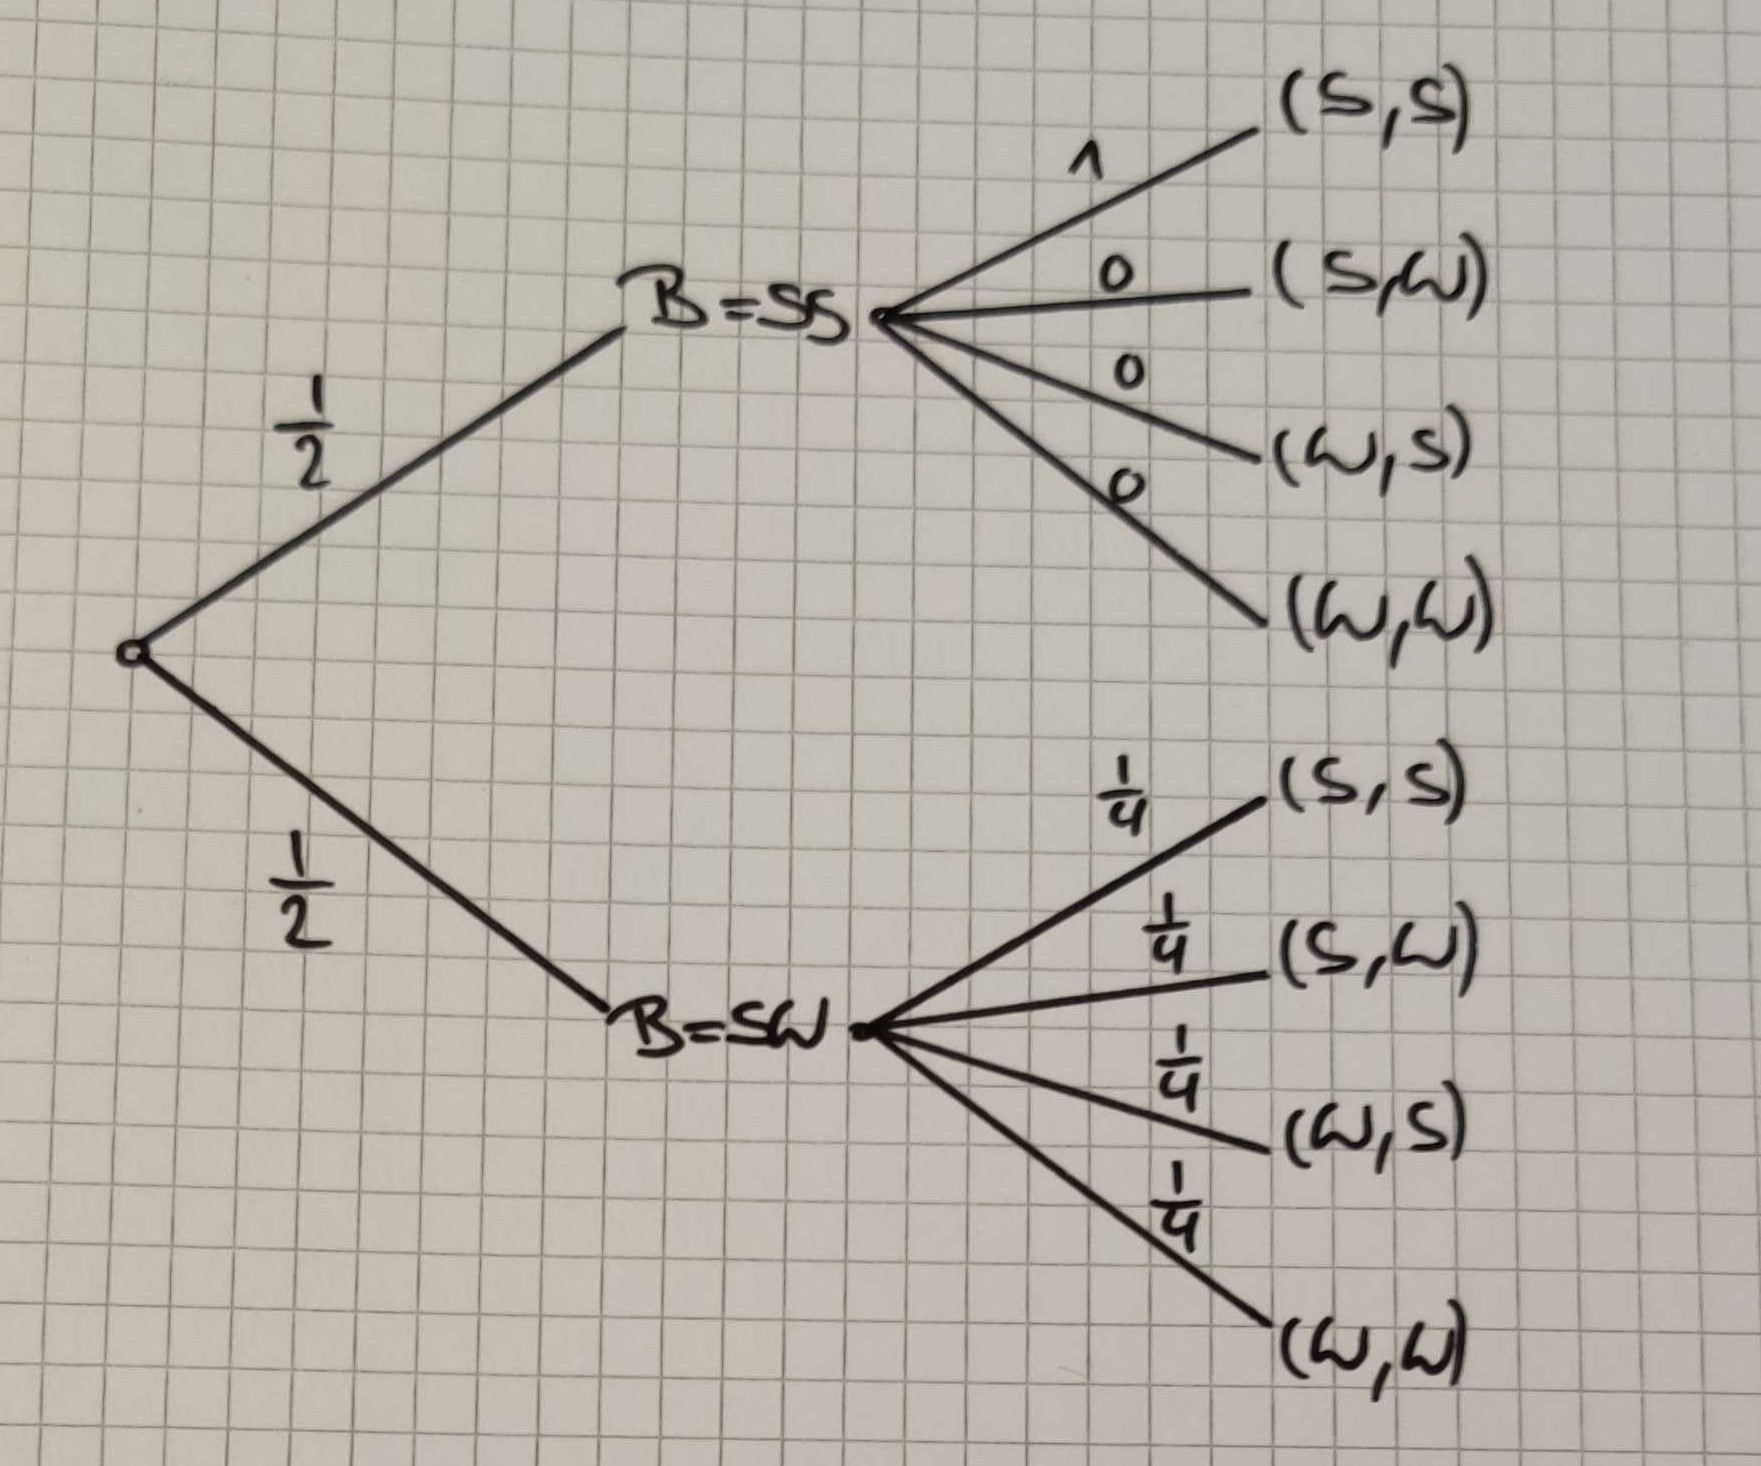
\includegraphics[width=100px]{img/MehrfachBaumVar2.jpg}
	\captionof{figure}{Variante 2 der Baum-Darstellung}
	\label{fig:Variante 2 der Baum-Darstellung}
\end{Figure}
\begin{equation}
\frac{P(B=SS, (S,S))}{P((S,S))}=\frac{0.5*1}{0.5*1+0.5*0.25}=\frac{4}{5}
\end{equation}
\section{Formelsammlung}
\subsection{von PDF zu CDF}
$f(x) = F'(x)$\\
$F(x) = P(X \leq x) = \int^x_{-\inf} f(x) dx$\\
f(x) $=$ PDF\\
F(x) $=$ CDF

\subsection{Erwartungswert}
$E(x) = \sum P(X=x_i) * x_i$\\
$E(x_1 + x_2) = E(x_1) + E(x_2)$\\
$E(x + \beta) = E(x) + \beta$

\subsection{Varianz}
$V(x) = \sum P(X=x_i) * (x_i - E(x))^2$\\
$V(x) = E(x^2) - E(x)^2$\\
$V(x + \beta) = V(x)$

\subsection{Bernoulli}
Kommt zum Zug, wenn es genau zwei Ergebnissmöglichkeiten gibt (bspw. Gewinn, Niederlage). Dabei gilt dann $x_i$ als Erfolgswahrscheinlichkeit. \\
$x_i = 0$ (Niederlage) $\rightarrow$ $1-P$\\
$x_i = 1$ (Gewinn) $\rightarrow$ P \\
Wobei wir für 0 und 1 jeweils den Wert einsetzen, welchen erzielt werden kann. Bspw. bei Niederlage -10 und bei Gewinn +1.
\textit{Bernoulli Erwartungswert}\\
$E(x_i) = p$ bzw. bei Mehrfachausführung $E(y) = n*p$ 

\textit{Bernoulli Varianz}\\
$V(x_i) = E(x_i ^2) + E(x_i)^2 = p - p^2 = p(1-p)$ bzw. bei Mehrfachausführung $V(y) = n * p * (1-p)$

\subsection{Formel für Wahrscheinlichkeit n von k Möglichkeiten (binominal)}
$P(x = k) = \binom{N}{K} * P^K (1-P)^{N-K}$\\
$N = $ Anzahl Durchführungen\\
$K = $ Anzahl Ereigniserfolg\\
$P = $ Einzelwahrscheinlichkeit\\
\textbf{ACHTUNG} ob mindestens, genau oder höchstens!

\subsection{Satz von Bayes}
\begin{equation}
	P(K|T) = \frac{P(T|K) * P(K)}{P(T)} = \frac{P(T|K) * P(K)}{P(T, K) + P(T, \bar{K})} = \frac{P(T|K) * P(K)}{P(T|K) * P(K) + P(T|\bar{K}) * P(\bar{K})}
\end{equation}

\begin{equation}
	P(\bar{K}|T) = \frac{P(T|\bar{K}) * P(\bar{K})}{P(T)} = \frac{P(T|\bar{K}) * P(\bar{K})}{P(T, K) + P(T, \bar{K})} = \frac{P(T|\bar{K}) * P(\bar{K})}{P(T|K) * P(K) + P(T|\bar{K}) * P(\bar{K})}
\end{equation}

\subsection{Diskret vs. Stetig}
stetig $\rightarrow$ Die Funktion / Linie ist durchgezogen und hat keine Unterbrechung\\
\textit{stetiger Erwartungswert}: $E(x) = \int^{\inf}_{\inf} f(x) * x dx$\\
\textit{stetige Varianz}: $V(x) = \int^{\inf}_{\inf} f(x) + x^2 dx - E(x)^2$\\
diskret $\rightarrow$ Verteilung ist punktuell bspw. bei Notenschlüssel
\textit{diskreter Erwartungswert}: $E(x) = \sum P(X=x_i) * x_i$\\
\textit{diskrete Varianz}: $V(x) = E(x^2) * x_i^2 - E(x)^2$\\ \textbf{bin mir nicht sicher ob Formel stimmt}




\end{document}